\chapter{Война и мир}

\section{Что ждет россиян во время частичной мобилизации?}
\textit{Источник: \url{https://lenta.ru/articles/2022/09/21/ukaz/}}

\textit{Ответы на главные вопросы}

Президент России Владимир Путин 21 сентября 2022 года объявил о введении в России \ed{частичной}{частичный}{partial} мобилизации. По его словам, призыву на военную службу подлежат граждане, состоящие в запасе, и прежде всего те, кто служил в армии. Кто теперь подлежит призыву, кто имеет право на \ed{отсрочку}{отсрочка}{delay; postponement}, каков порядок мобилизации — в этих вопросах разбиралась «Лента.ру».

\ed{Указ}{ук\'{а}з}{decree} «Об объявлении частичной мобилизации в Российской Федерации» опубликован на сайте Кремля в среду, в 9 часов 20 минут.

«Объявить с 21 сентября 2022 года в Российской Федерации частичную мобилизацию», — сообщается в первом пункте документа, подписанного президентом России Владимиром Путиным.

Во втором пункте указано, что мобилизованные граждане получат статус военнослужащих-контрактников с денежным содержанием соответствующего размера. Увольнение из рядов мобилизованных предусмотрено только по возрасту и по состоянию здоровья.

Правительству поручено финансировать мероприятия по проведению частичной мобилизации, главам регионов — обеспечить призыв находящихся в запасе граждан.

\textbf{Сколько человек призовут?}

Согласно заявлению главы Минобороны Сергея Шойгу — 300 тысяч. Это примерно 1,1 процента от общего мобилизационного ресурса России, который, по словам министра, составляет почти 25 миллионов человек. Для каждого региона количество подлежащих мобилизации будет определяться отдельно.

\textbf{Кого призовут в первую очередь?}

По словам Шойгу, на военную службу по мобилизации будут призваны те, кто отслужил в армии, имеет военно-учётную специальность и соответствующий опыт. Перед отправкой в части они пройдут обязательную дополнительную подготовку.

\ed{Полковник}{полковник}{colonel (army)} \explain{в отставке}{retired} Виктор Баранец считает, что первыми под мобилизацию попадут резервисты, которые каждый год по указу президента призывались на военные сборы, стреляли, водили танки и наводили ракеты. Кроме того, будут призваны люди, по разным причинам уволенные с контрактной службы, а также молодые офицеры.

«Резервисты -- это \explain{военнообязанные}{conscripts; liable for military service} граждане государства, которые подлежат мобилизации при необходимости, -- рассказал в свою очередь «Ленте.ру» \explain{судь\'{я}}{judge} в отставке Владимир Комсолев. —- В нашем случае это лица, прошедшие службу и имеющие достаточную подготовку. Они заключили контракт о пребывании в резерве и получают за это деньги. Раз в год резервисты выезжают на военные сборы, раз в месяц участвуют в занятиях».

Юрист Артем Мугунянц в разговоре с «Лентой.ру» отметил, что тех, кто пользовался отсрочкой в период с 18 до 27 лет и не служил, мобилизация, вероятно, не коснётся.

«Мобилизации подлежат только те, кто служил в армии либо офицером, либо проходил срочную службу, либо был контрактником\footnote{Only those who served in the army either as an officer, or did military service, or were a contract soldier \textit{are subject to} mobilization}. — пояснил эксперт. — Можно предполагать следующее. Так как утверждается, что необходимо освобождать территории Украины, им потребуются \explain{наступательные войска}{offensive troops}: танкисты, \explain{морская пехота}{marines}, мотострелковые части. Эти части и войска могут потребоваться в большом количестве. Тех, кто служил в этих войсках, будут мобилизовать в первую очередь».

\textbf{Людей какого возраста могут призывать?}

Согласно статье 53 Федерального закона «О воинской обязанности и военной службе», все военнослужащие запаса делятся на три разряда. В случае мобилизации первым в ВС попадает первый разряд, затем — второй, третий — последним (подробнее о том, что значат категории запаса и категории здоровья — ниже).

По первому разряду призываются солдаты и низшие \ed{чины}{чин}{rank} в возрасте до 35 лет, младшие офицеры в возрасте до 50 лет (в третьем разряде верхние рамки для этих званий повышаются до 50 и 60 лет соответственно) и так далее. Представители генералитета подлежат мобилизации по второму разряду в возрасте до 70 лет.

В Госдуме заявили, что планируют призывать тех, кто попадает под первый разряд.

«Пока человек не снят с военного учёта, он может подлежать мобилизации, — пояснил «Ленте.ру» профессор кафедры уголовного права РГПУ имени А.И. Герцена Сергей Милюков. — Есть специальности в ближнем и дальнем тылу, где возраст не является большой \ed{пом\'{е}хой}{пом\'{е}ха}{hindrance}. Например, обязательно потребуются медики. Призванные врачи будут оказывать медпомощь в госпиталях в тылу. Для лечения и \ed{дол\'{е}чивания}{дол\'{е}чивание}{follow-up treatment} нужно привлечь санатории, как это было в Великую Отечественную войну. Непосредственно же в боестолкновениях должны участвовать более молодые люди».

\textbf{Что означают категории запаса и категории здоровья в военном билете? }

Существует пять категорий годности к военной службе. Их определяют исходя из показателей здоровья и записывают данные об этом в военном билете.
\begin{itemize}
    \item «А» — \explain{годен}{fit} к военной службе;
    \item «Б» — годен к службе с \ed{незначительными}{незначительный}{insignificant} ограничениями;
    \item «В» — ограниченно годен к военной службе;
    \item «Г» — временно не годен;
    \item «Д» — не годен к несению военной службы.
\end{itemize}
Группы здоровья «А», «Б» и «В» по федеральному закону \explain{подлежат}{are subject to} мобилизации.

Всех резервистов \ed{распределяют}{распределять}{distribute} по трем категориям в зависимости от возраста военнослужащего и полученного звания.

Первая категория — граждане, которых призывают в первую очередь в случае мобилизации. \explain{Речь идет о}{This is a very useful expression; it means ``this is about...''} военных, которые не получили офицерский чин (в том числе \ed{прапорщики}{прапорщик}{ensign} и мичманы) и не \explain{перешагнули}{stepped over} возрастной \explain{пор\'{о}г}{threshold} в 35 лет, а также о младшем офицерском составе до 45 лет (лейтенант, капитан). В данной категории числятся старшие офицеры до 50 лет (майор, \explain{подполковник}{lieutenant colonel}); полковники, капитаны 1 ранга до 55 лет; высшее руководство до 60 лет. Первым на службу должен прибыть офицерский состав высшего эшелона.

Вторая категория — военнообязанные старшей возрастной группы или те, кто не прошел в первую волну мобилизации по здоровью. В эту группу попадают солдаты, военнослужащие без офицерского звания в возрасте от 35 до 45 лет, младший руководящий состав от 45 до 50 лет и старшие офицеры от 50 до 55 лет.

Третья категория — военнослужащие, которых призывают только в том случае, если военные действия длятся больше года и необходимы дополнительные силы. Под эту категорию попадают \explain{рядовые}{privates} и \explain{матросы}{sailors}, прапорщики и мичманы самой старшей возрастной категории. Возраст низшего\footnote{низкий, низшего} офицерского состава этой категории до 55 лет, а для капитанов 2 и 3 ранга и подполковников — до 60 лет. В данной категории пребывают военнообязанные женщины в возрасте до 50 лет.

\textbf{Что такое мобилизационное предписание? }

Это документ, который выдается части запасников. Выдача мобилизационного предписания — это \explain{своеобразная}{peculiar, singular, sui generis} перепись военнообязанных лиц. Гражданин, который получил мобилизационное предписание, при объявлении мобилизации должен прибыть в указанное в нем место и срок без дополнительной \ed{повестки}{повестка}{subpoena, writ} и предупреждения.

Как \explain{утверждает}{claims} юрист Павел Чиков, во время мобилизации гражданам приходят повестки, как и в обычное время — лично в руки или под подпись. Повестку также могут вручить по месту работы.

Однако именно запасники, имеющие мобилизационные предписания, по статье 21 ФЗ «О мобилизационной подготовке и мобилизации в Российской Федерации» самостоятельно должны \explain{явиться}{show up} в военный комиссариат.

\textbf{Кто имеет право на отсрочку?}

Как следует из указа, подписанного Путиным, \ed{отсрочку}{отсрочка}{postponement} пол\'{у}чат работники оборонных предприятий. «\explain{Предоставить}{provide} гражданам Российской Федерации, работающим в организациях оборонно-промышленного комплекса, право на отсрочку от призыва на военную службу по мобилизации (на период работы в этих организациях). Категории граждан Российской Федерации, которым предоставляется право на отсрочку, и порядок его предоставления определяются правительством Российской Федерации», — говорится в документе.

Как следует из статьи 18 федерального закона о мобилизации, отсрочка также предоставляется:

\begin{itemize}
    \item временно \ed{негодным}{негодный}{ineligible, not qualified} к военной службе по состоянию здоровья;

    \item ухаживающим за близкими родственниками, которых больше некому содержать;

    \item многодетным родителям (тех, кто имеет на \ed{иждивении}{иждив\'{е}ние}{dependent} не менее четырех детей в возрасте до 16 лет или троих детей при условии беременности супруги сроком не менее 22 недель);

    \item родителям-одиночкам;

    \item членам Совета Федерации и депутатам Госдумы.
\end{itemize}

Другие категории военнообязанных, которым \explain{полагается}{depends, relies} отсрочка (бронь от призыва), еще не известны. Их определяет правительство России, напомнил пресс-секретарь президента Дмитрий Песков.

\textbf{Попадают ли под мобилизацию срочники и те, кто не служил в армии? }

По закону о мобилизации — не попадают. Из него следует, что в ряды вооруженных сил должны быть направлены «граждане, пребывающие в запасе, не имеющие права на отсрочку от призыва на военную службу по мобилизации».

По словам юриста Ольги Лютницкой, \explain{срочники}{conscript} не попадают под эту категорию, так как они еще не переведены в запас.

Если гражданин не служил, например, потому, что был ограниченно годен, но у него есть военный билет, то веротность его мобилизации есть, сказала она «Ленте.ру».

Юрист Мугунянц уточнил, что срочники уже являются военнослужащими по призыву. Задействовать их до объявления полной мобилизации и войны нельзя.

\textbf{Можно ли мужчинам теперь выезжать за границу? }

В Федеральном законе «О мобилизационной подготовке и мобилизации в Российской Федерации» говорится, что «гражданам, состоящим на воинском учете, с момента объявления мобилизации воспрещается выезд с места жительства без разрешения военных комиссариатов, федеральных органов исполнительной власти, имеющих запас».

Юрист Лютницкая утверждает, что пока по вопросу \ed{запрета}{запрет}{ban, prohibition} выезда мужчинам за границу нет никаких законодательных актов и комментариев. Поэтому прямо сейчас никаких ограничений для выезда не существует.

Юрист Мугунянц также отметил, что выезжать никому не запрещено: выезд закрывается только при полной мобилизации.

«Если же человека мобилизовали, то есть признали военнослужащим, дали мобилизационное предписание о том, что он должен явиться, то он действительно не может выехать в другую страну. Потому что он мобилизован», — уточнил эксперт.

При этом скорее всего человека не будут вносить в каике-либо базы, но гражданин должен \explain{учитывать}{take into consideration}, что выезд будет расценен как \explain{уклонение}{evasion} от армии, за которое возникнут соответствующие \explain{уголовные последствия}{criminal implications}.

Член Совета по правам человека при президенте России Кирилл Кабанов заявил, что для людей без повесток на руках юридического запрета на выезд за границу нет.

\textbf{Что ждет тех, кто по достижении 27 лет получил справку вместо военного билета?}

Те, кто не проходил службу в вооруженных силах \explain{без уважительной причины}{without good reason} (например, сознательно \ed{уклонялся}{avoided, dodged}), и по достижении 27-летнего возраста получил справку \explain{взамен}{instead of} военного билета, вероятно, не будут призваны во время частичной мобилизации, так как они тоже — не служившие люди, считает юрист Мугунянц.

«На данном этапе у них никаких проблем нет. Если объявят всеобщую мобилизацию, то [обладателей справок] будут призывать, как и всех. К ним будут применяться те же условия, как к людям, которые не служили, но имеют военный билет. То же касается и тех, кто вообще не имеет никаких документов [подобного рода]. Важно, что они находятся в мобилизационном возрасте и подпадают под [всеобщую] мобилизацию».

По российскому законодательству, обладатель справки не может быть принят на государственную службу, в остальном его права не отличаются от прав владельца военного билета.

\textbf{\explain{Затрагивает}{affects} ли мобилизация женщин?}

По закону, мобилизация граждан, пребывающих в запасе, \explain{предполагает}{suggest} возможность призыва на военную службу медработников женского пола в возрасте до 45 лет. У них на руках есть военные билеты — медработники получают их после учебы.

Адвокат Владимир Шелупахин объяснил «Ленте.ру», что призыв состоящих на воинском учете женщин предполагается только в третью очередь, то есть после мужчин в возрасте 35-45 лет, в том числе граждан, пребывающих в запасе, но годных к военной службе с незначительными ограничениями (категория «Б») или ограниченно годных к военной службе (категория «В»).

«\ed{Вовсе}{вовсе}{at all} \explain{освобождаются}{released} от службы матери-одиночки и многодетные матери», — добавил юрист. Кроме того, на женщин распространяются и другие отсрочки, описанные в федеральном законе.

\textbf{Могут ли повестки приходить через «Госуслуги»?}

По официальной информации — нет. О возможной отправке повесток через сервис \ed{Госуслуг}{Госуслуги}{public services} 21 сентября написал Telegram-канала Baza. По информации издания, всем, кого собираются призвать, придет уведомление в аккаунте Госуслуг дополнением к обычным повесткам через почту.

Однако в Минцифры почти сразу это \explain{опровергли}{refuted}. «В связи с появившимися в соцсетях публикациями о том, что электронные повестки в рамках частичной мобилизации будут \explain{рассылаться}{be sent out} через Госуслуги, сообщаем, что таких планов нет. Необходимая законодательная база для этого отсутствует», — говорится в Telegram-канале министерства.

\newpage
\section{Таких замученных людей я раньше не видел}

\textit{Рассказ россиянина, который несколько суток пытался уехать в Казахстан }

\textit{Источник: \url{https://baza.io/posts/4250c126-5344-458d-af97-21179596c136}}

Сутки на жаре и холоде, драки, голод и бессонница. Со всем этим столкнулся Александр, который после объявления о «частичной мобилизации» решил уехать на машине в Казахстан. Однако там его, как и тысячи других россиян, встретил своеобразный тест на выживание и целый ряд гуманитарных проблем.

Это детальный рассказ Александра о том, что сейчас происходит на границе с Казахстаном в Астраханской области.


\textbf{Добраться до границы}

Мчались к границе под Астраханью в режиме аврала: за ночь собрали чемоданы, бросили ключи от квартиры с котом друзьям и полетели в Волгоград, так как только туда в эти дни были нормальные цены на билеты. Самолёт был полностью забит мужчинами. Когда заходил, услышал, как одна бортпроводница шепнула другой насчёт пассажирки: «О, девушка, ничего себе! Впервые за два дня».

Уже в самолёте стало ясно: ехать, как мы планировали, на поезде до Астрахани очень долго, и потому прямо в аэропорту взяли таксиста. Спросили, за сколько он довезёт до границы под Астраханью, и он, назвав сумму в 15000, сразу получил её в руки. Мы гнали больше ста весь путь. В какой-то момент водитель даже чересчур заспешил и чуть не размазал нас по встречной фуре.

Остановились только один раз — на пустынной заправке у трассы. Там был заправщик, который принялся нам угрожать и затевать драку из-за того, что мы бежим из страны. Мы ничего ему не говорили, но ему было очевидно, что мы москвичи, так как он обронил «из-за таких, как вы, у меня всех братьев забрали».

Обидно было, что он именно нас в этом обвиняет, а не власть. Но вместе с тем жалко парня: многим очевидно, что в сёлах больше пропорции набора.


\textbf{Звёзды и безысходность под Астраханью}

Подобрались к границе Астрахань — Атырау с наступлением темноты, тогда длина пробки до КПП была уже 14,9 километра. Там уже царила анархия: нам с ходу предложили купить велосипед за 50000 рублей, на котором можно было проехать границу. Далее следовал жуткий марш-бросок в кромешной тьме с чемоданами под дождём в дикий холод: вместе с тьмой на пробку опустилась осенняя прохлада и ливень.

Мы прошли вместе с чемоданами около 8 километров, разглядывая, как люди друг с другом ругаются из-за мест, как плачут уставшие дети в машинах, как кричат кошки в переносках. Люди пытались лечь спать в совершенном аду. Над нами, стоит отметить, висело фантастически красивое звёздное небо: в радиусе километров не было огней, и это был фантастический вид на звёзды. Но вместе с тем впервые пришло отчаяние: стало понятно, что выжить тут будет нереально.

Вокруг сновали люди на велосипедах с подвязанными к спине чемоданами, люди на гироскутерах, самокатах, местная банда бородатых наглецов, отжимавших места поближе к границе на продажу, и огромная, невообразимая по длине пробка из легковых и большегрузных машин, у которой не было конца. Спустя два часа такого движения, не найдя конца очереди, мы устали смертельно, и пришло понимание: либо мы сейчас едем в аэропорт и домой, либо должны немедленно устроиться на ночлег. Я был замерзший, мокрый и абсолютно раздавленный безысходностью.

И тут я увидел паренька лет 20, который ехал один в этой пробке на своей машине. Ходили слухи, что пробку на машине можно преодолеть только за сутки-полтора, и я удивился: как он в одиночку, без смены собирался ехать такой период времени без остановки? Мы предложили ему за деньги взять нас до границы, пообещав подменять за рулём для сна. Парень согласился, и мы залезли в машину. Боже, как было уютно и тепло после холодной дождливой улицы! Мы часа три-четыре ехали с ним, стараясь лавировать между дальнобойными машинами, которые пытались блокировать дорогу бомбилам, занимающим места. При этом мы весело болтали за жизнь. Стало понятно, что компания приятная.

Я чувствовал, что дико устал. Время уже было около часа ночи, как вдруг движение встало. Перед нами была вереница дальнобойщиков, уходящая в бесконечную даль, и мы в ожидании, когда вновь начнётся движение, заглушили двигатель и в какой-то момент уснули.


\textbf{«Голодные игры»}

Я проснулся спустя пару часов: было холодно даже внутри машины, хотя спал я в куртке. Парень, который нас взял, курил возле авто, закутанный во всю одежду, что у него была. Мы стояли окружённые со всех сторон дальнобойщиками, которые спали в кабинах. А вокруг был шум двигателей. Казалось, все едут, и только мы стоим в своём маленьком дальнобойном ряду.

Парень сходил на разведку и вернулся с криком «Погнали!». На часах было только 4 утра, и тьма была непроглядная. Мы очень аккуратно вылезали между дальнобойщиками на обочину и, когда выехали, увидели сцену из какого-то плохого спин-оффа фильма «Голодные игры»: сотни автомобилей носятся по полю, пытаясь обогнать друг друга в пробке на дороге и влезть где-то ближе к первому блокпосту ГИБДД.

Мы вместе со всеми выехали на поле и оказались в абсолютной мясорубке: ночь, вой моторов и сотни водителей, выдавливающих друг друга с дороги в кювет. Уже не знаю, как у паренька это вышло, но благодаря своей наглости и терпению он нашёл небольшой перекрёсток с просёлочной дорогой, чтобы вклиниться, и мы заняли позицию до рассвета.


Рассвело к шести, и на перекрёстке появился сотрудник ГИБДД. Он пытался разрулить весь тот кошмар, который произошёл за предрассветные часы. Водителей, ждущих в пробке уже сутки, это злило: кто-то за ночь влез без очереди из-за дальнобойщиков, которые заблокировали поток в знак отместки за потерянное время. Теперь такие водители не давали сотруднику ГИБДД пропускать влезшие с обочины машины.

Инспектор был абсолютно уставший и измождённый и в какой-то момент просто ушёл, оставив всё это дело жить своей жизнью. А жизнь была такая: пока на горке совершали намаз мусульмане, семьи с детьми пытались умыть уставших и невыспавшихся детей, а кто-то гулял с собакой, привезённой с собой в этот кошмар.

«Нам тут не влезть», — хмуро сказал наш водитель, и мы пошли искать сообщников на прорыв. Картина открывалась жуткая. Поговорив с окружающими, мы узнали, что люди, стоявшие в честной пробке, провели здесь уже сутки, тогда как наш маршрут занимал около 10 часов. Многие были с детьми, пожилыми родителями, животными. Кто-то из них набрал попутчиков. Но всех объединяло одно: все они, так же как и мы, ночью были заблокированы колонной дальнобойщиков.

Услышав шум машин и оскорбившись такой наглостью, водители бросились объезжать их по полям, перемешивая все очередности. Этот перекрёсток был всего в 5 километрах от границы.


\textbf{Банка майонеза, драки и ФСБ}

В пробке было много машин с Северного Кавказа: с номерами из Дагестана, Чечни, Ингушетии. Они везли семьи, детей, родителей: их семьям угрожало наказание за то, что они уклоняются от мобилизации, потому всех брали с собой. Здесь же были и напуганные студенты, и взрослые мужчины, и ребята со всей страны: Ростовской, Краснодарской областей, попадался Санкт-Петербург и Карелия. Представьте, люди приехали сюда из Карелии!

Куда, спрашиваю у водителя, здесь ходят в туалет? Он смеется: «А как ты думаешь? Спустись с дороги». И тут я увидел страшное зрелище: отходить от дороги далеко нельзя — вдруг твоё место займут? Тех, кто ушёл дальше 50 метров, разворачивали пограничники. Поэтому люди были вынуждены ходить в туалет прямо здесь, на глазах всей пробки. Десятки тысяч людей, женщин, мужчин, любых вероисповеданий и культур. Все делали это здесь.

Обстановка накалялась: люди не могли поделить дорогу, и вспыхивали драки в разных частях пробки. Солнце окончательно поднялось, и стало жарко. Ещё ночью ты заворачивался во все вещи из чемодана, а сейчас потел в футболке.

Стало понятно, куда уехал сотрудник ГИБДД: он вернулся с группой пограничников и бойцами ФСБ на «Барсе». Они подняли оружие, будто угрожая начать пальбу в воздух, но толпу это мало пугало: несколько ретивых ребят попытались втянуть в драку инспектора. Только с появлением майора ГИБДД — уставшего, с выгоревшей на солнце кожей и грозным голосом — удалось сбить накал и договориться о системе проезда. Разумеется, и она не соблюдалась. Как только инспектор принимался разруливать проблему в одной точке пробки, вспыхивали бои в другой.

Мы смогли въехать на точку, указываемую в многотысячных чатах пробки как ключевую, после которой «ад заканчивается» и «всё становится интеллигентно». Здесь находился узкий мост, и далее авто двигались в образовавшейся колонне одна за другой. Ну как двигались: за 12 часов все продвинулись на 600–700 метров, не более.

Тут появилась гуманитарная проблема: у кого-то заканчивалось топливо, у кого-то еда и вода для детей и взрослых. Некоторые были отправлены в город за едой, но тут же попадали в капкан: их машины не хотели пропускать обратно в задней части пробки, и эти машины выбывали из общей гонки.

К этому времени о пробке уже трубили СМИ. Новости от тех, кто был на границе, расстраивали: они стояли по трое суток. Мы достигли посёлка, в конце которого находился КПП, только к темноте. В посёлке в это время совершенно опустел магазин: только одинокая банка майонеза стояла в пустом холодильнике. Проблема с водой, едой и топливом решена не была: люди в моей части колонны делились этим с соседями, некоторые продолжали толкать машину, чтобы не заводить авто и не тратить топливо. Я отдал две из трёх оставшихся бутылок воды в соседние машины с детьми, а также раздал большую часть своей аптечки. Особенно было популярно обезболивающее.


Обочина в этой части была полна мусора от наших предшественников, а также сбежавшимися на него собаками. Это отпугивало людей от туалета. Еда почти у всех кончилась, наступила ночь, и снова стало холодать.

На помощь пришли жители посёлка. Они за крайне низкие цены стали продавать еду, заряжать телефоны, бесплатно пускать в туалет, а детей — отдохнуть в дома. Но вместе с темнотой пришла и новая проблема: организованные «мафиози» держателей мест вклинивались в ряды. Их целью было удержать позицию в этой части пробки и продать их тем, кто прибыл в конец.

По слухам, место в этой части пробки стоило по 25–30 тысяч рублей. Это приводило к конфликтам и дракам, маханию ножами и угрозам убийством. На самые громкие драки прилетали сотрудники ФСБ на «Барсе», в балаклавах и с автоматами. Это успокаивало конфликтующих — до отъезда офицеров.


\textbf{Дорожная «мафия»}

Здесь, в 4 километрах от границы, уже было много пешеходов с сумками. Они доходили до этой части колонны и просились в машины: переходить границу пешком было нельзя. У обочины были свалены велосипеды: люди, накупившие их в конце пробки за 30–50 тысяч рублей, у КПП узнавали, что на велосипеде было всё-таки нельзя. Пеших кто-то подсаживал бесплатно, а кто-то брал за деньги. И тут начался новый коллапс: каждый, кто слышал о более высокой цене, поднимал цену у себя, и в итоге стоимость места в машине выросла до 40–50 тысяч рублей.

Чем темнее становилось, тем активнее начинались бои во второй части «Голодных игр». Вместе с этим накопилась усталость: за двое суток, из которых на сон пришлось 3 часа, мы не выспались. Первоначальный план, согласно которому мы хотели меняться местами с водителем, разбился о необходимость вылетать из машин по свисту — для обороны мест от влезавших барыг-продавцов. Это длилось всю ночь.

Третьи сутки прошли по абсолютно такому же сценарию, но изменились цены: мы были уже в 2 километрах от КПП, и цены на места для пассажиров достигали 70 тысяч. Еда и вода стали дефицитными, мы совсем отказались от еды в пользу детей, водой нас снабжали местные жители совершенно бесплатно. Для экономии топлива многие стали толкать машины. Чтобы хоть как-то спать, часть не умеющих водить пассажиров освоили основы вождения.

К ночи началась третья серия «Голодных игр» с ещё более активным противостоянием. Здесь уже оставалось менее 500 метров до КПП, и дорога была блокирована десятками мужчин, утверждавших, что это их территория, а машины будут пропускаться по системе «шесть из колонны — одна их».


«Одна их» представляла собой минивэн с вместимостью 6–12 человек, куда сажали пешеходов по цене от 70 до 90 тысяч рублей за место. На дороге появились «служебные машины» с сопровождением ГИБДД, следовавшие в сторону КПП. В числе служащих были замечены пожилые женщины и подростки. Обратно они не возвращались.

Бои длились до утра. Под эффектный рассвет мы пересекли КПП. Там все уже были знакомы: сотрудники ФСБ, помогавшие отвоёвывать места, пограничники, с уставшими лицами проезжавшие мимо пробки на микроавтобусе, работники ГИБДД, нервно курившие после изнуряющей смены в ночном кошмаре.

На КПП были и молодые люди, которых задержали в связи с тем, что они получили повестки. Стало ясно, что слухи о списках на границах вовсе не были слухами.


\textbf{Переход}

Под встающее солнце мы с уже родными соседями пересекали границу и неслись по буферной зоне, в которой, как нам завещали сотрудники российской погранзаставы, не стоит покидать автомобиль. Проехав шесть километров из двенадцати, мы уткнулись в новую пробку.

У буферной зоны была особенность: здесь не было ни сотрудников ГИБДД, ни ФСБ. Зато были свои барыги: они перевозили людей за 30–50 тысяч от одного КПП до другого через встречную полосу. Здесь они были более подготовлены и ездили по двое, с охраной. Но и люди, попавшие в эту зону, были уже ветеранами и прямо между двумя погранзаставами мастерили себе примитивное оружие близкого боя. Как ни странно, боёв не было. Но день прошёл в столкновениях и наездах машин барыг на активистов пробки.

Моторы здесь не заводились, даже для движения в горку, пить воду перестали даже женщины, кто-то набирал воду из местной реки, которая оказалась достаточно чистой. Не было слёз и истерик: к четвёртым суткам погранперехода плакать уже не умели, лишь сурово грустить. Я был знаком с людьми на десятки машин назад и вперёд: отличные ребята со всей европейской части страны, бегущие от правительства и безысходности.

Организовывались сигналы тревоги и группы быстрого реагирования для непропуска барыг. Дальнобойщики, чудом прорвавшиеся в эту зону, грели воду для бытовых нужд: некоторые впервые за эти дни чистили зубы или умывались. На реке появилась лодка: в ней приплыла семья из республики Северного Кавказа, пересекшая таким образом границу: они бесплатно раздавали всем еду, воду и лекарства.

К ночи приехали российские пограничники. Они строго запретили покидать автомобили: таковы были правила проезда. Исключения сделаны были для тех, кто толкает машины. К глубокой темноте мы прошли мост — переход через границу и встали в очередь к казахскому КПП.

Последний этап этого квеста был связан с полным отсутствием сил. Без еды, сна и покоя мы провели по четверо суток. Впереди было ещё шесть часов в пробке. Появился интернет, а вместе с ним в чате пробки появилась информация о местах в машине по 150000 рублей и барыгах, которые перевозили людей в нейтральную буферную зону за одну сумму, а уже в буферной зоне требовали другую. Те, кто не соглашался, отправлялись обратно.

Водители засыпали за рулём: сказывались по 80–96 часов без отдыха. Все были измождены и глубоко несчастны. Казахские пограничники встречали людей сочувствием и крайне лояльным досмотром. Впервые показалось, что мы действительно беженцы: таких несчастных и замученных людей я раньше не видел.

Впереди у нас было ещё шесть часов по бездорожью в степи до ближайшего города.


\newpage
\section{Народ — президент — Бог}


\textit{Зачем «военное духовенство» РПЦ заменяет Евангелие Ветхим Заветом, а \explain{з\'{а}поведь}{commandment} о любви — заповедью об уничтожении врагов }

\textit{Александр Солдатов, обозреватель «Новой газеты»}

\textit{Источник: \url{https://novaya-media.cdn.ampproject.org/}}

Православный федеральный телеканал «Спас» выпустил цикл передач «Война и Библия». Главный редактор телеканала Борис Корчевников в сопровождении настоятеля храма РПЦ при МГИМО протоиерея Игоря Фомина, позируя в полной военной экипировке, продвигают такую трактовку библейских сюжетов, которая, по их мнению, полностью объясняет происходящее. Вышло уже пять серий цикла, основной набор идей повторяется в каждой из них: «СВО» имеет сакрально-мистический характер; на стороне Украины сражаются еретики и сатанисты, а российская армия исполняет заповеди, данные еврейскому народу при исходе из Египта, когда он покорял Палестину — Землю обетованную, истребляя населявшие ее народы.

Мистический крен в российской пропаганде возник в октябре — на фоне кризиса первоначальных целей «спецоперации» («демилитаризация» и «денацификация») и усилился на фоне частичной мобилизации. Хотя религиозность россиян (особенно мужского населения) не очень высока, власть вынуждена обращаться к религиозной риторике — с ее помощью формируется некая синкретическая религия, которая игнорирует различия, например, между православием и исламом, акцентируя внимание на «духовной несовместимости» Запада и России.

Представляя основные постулаты этой религии, помощник Николая Патрушева Алексей Павлов заявил: «С продолжением специальной военной операции становится все более насущным проведение десатанизации Украины, или, как метко выразился глава Чеченской Республики Рамзан Кадыров, ее «полной дешайтанизации».

Развивая этот тренд, Дмитрий Медведев наделил РФ, олицетворяемую президентом, божественными свойствами: «Мы приобрели сакральную силу, — заявил он. — У нас есть возможность отправить всех врагов в геенну огненную». И сформулировал новую цель «СВО»: «Остановить верховного властелина ада, какое бы имя он ни использовал — Сатана, Люцифер или иблис».

\begin{fancyquotes}
    Медведев угрожает украинцам словами из ветхозаветного пророчества Иезекииля: «Не пощадит тебя око Мое, и не помилую. По путям твоим воздам тебе, и мерзости твои с тобою будут; и узнаете, что Я Господь каратель» (Иез. 7:9).
\end{fancyquotes}

В отличие от Евангелия, которое, как утверждает Коран (2:75; 4:46; 5:13, 41), христиане «исказили», Ветхий Завет — священные книги еврейского народа, написанные до пришествия в мир Христа, — равно почитаются христианами и мусульманами. В исламской традиции они известны как «ат-Таурат». В этом контексте неудивительно, что авторы цикла «Война и Библия» апеллируют именно к Ветхому Завету. В 4-й серии они смакуют историю истребления семи народов при завоевании Палестины еврейским воинством под предводительством Иисуса Навина.

Ведущий Борис Корчевников называет заповедь «Пойди и вырежи весь народ» великим испытанием веры. А протоиерей Игорь Фомин ополчается на либералов, которые считают, что «даже правитель не может лишать жизни». «Но Священное Писание, — утверждает воинствующий служитель, — говорит совершенно об обратном».

Подмена тут заключается в том, что христиане имеют другое Писание! Точнее, ключом для понимания Писания у христиан служит Евангелие, а у православных — еще и тысячелетняя святоотеческая традиция его толкования. Иисус Христос в Евангелии часто цитирует заповеди Ветхого Завета, но почти каждый раз предлагает совершенно новое, духовное их понимание. Вспомним Нагорную проповедь: «Сказано древним: не убивай, кто же убьет, подлежит суду. А Я говорю вам, что всякий, гневающийся на брата своего напрасно, подлежит суду… Сказано древним: не \ed{прелюбодействуй}{прелюбодействовать/спрелюбодействовать}{to commit adultery}. А Я говорю вам, что всякий, кто смотрит на женщину с \ed{вожделением}{вожделение}{страстное желание; сильное чувственное влечение (lust)}, уже прелюбодействовал с нею в сердце своем\dots Сказано: око за око и зуб за зуб. А Я говорю вам: не противься злому. Но кто ударит тебя в правую щеку твою, обрати к нему и другую… Сказано: люби ближнего твоего и ненавидь врага твоего. А Я говорю вам: любите врагов ваших, благословляйте проклинающих вас, благотворите ненавидящим вас и молитесь за обижающих вас и гонящих вас» (Евангелие от Матфея, глава 5).


\begin{fancyquotes}
    Евангелие — самая неудобная книга в современных реалиях.
\end{fancyquotes}

Встречаясь с военным духовенством 1 декабря в храме Христа Спасителя, патриарх Кирилл также не цитировал эту неудобную книгу. Он \ed{восхвалял}{восхвал\'{я}ть/восхвал\'{и}ть}{to praise} \ex{доблесть}{\textit{высок.} высшая добродетель (virtue); стойкость; высшее мужество, готовность преодолеть препятствия для достижения какой-либо высокой цели, самоотверженность в какой-либо деятельности} тех, кто «с оружием в руках защищает родину», и выражал надежду, что поездки духовенства на фронт «закалят» священников. Патриарх намерен «циркулярными письмами» направлять туда все новые и новые партии духовенства. В своей потрясшей христианский мир проповеди 25 сентября он автоматом признал попавшими в рай всех российских воинов, погибших на полях Украины: по его мнению, такая гибель «смывает все грехи, которые человек совершил».

\begin{fancyquotes}
    «Идите смело исполнять свой воинский долг, — напутствовал Кирилл воинов. — Если вы жизнь положили за родину ``\dots'', то вы будете вместе с Богом в Его Царствии».
    Евангелие содержит совсем другие «напутствия воинам».
\end{fancyquotes}

«Возврати меч твой в его место, ибо все, взявшие меч, мечом погибнут» (Мф. 26:52), — говорит Христос апостолу Петру, пытавшемуся защитить Учителя от ареста (об истории толкования этого места Евангелия рассказывала «Новая»). «Наша война не живых делает мертвыми, а мертвых — живыми, изобилуя \ed{кротостью}{кротость}{свойство по значению прилагательного кроткий; добродетель, заключающаяся в уклонении от проявления гнева и ярости; уступчивость, покорность, смиренность (meekness)} и великим смирением, -- говорил святитель IV в. Иоанн Златоуст о духовном понимании ветхозаветных сюжетов о войне (\url{https://religion.wikireading.ru/amp190553}). — \ed{Мне привычно}{мне привычно}{I'm used to} терпеть \ex{преследование}{pursuit}, а не преследовать, быть гонимым, а не гнать. Так и Христос побеждал, не распиная, а распятый, не ударяя, но приняв удары».

«Народ — президент — Бог», --- торжественно декламирует новую русскую «триаду» протоиерей Игорь Фомин. Она рефреном \ex{пронизывает}{pervades} цикл «Война и Библия», апеллируя прямо к подсознанию зрителей, убеждая в том, что все три реальности вечны и бессмысленно возражать или сопротивляться им. Главный посыл этих грубых намёков --- президент \ed{непогрешим}{непогрешимый}{не совершающий ошибок, не ошибающийся (infallible)}, даже если большинству его подданных непонятен смысл самого важного решения всей его жизни, а может быть, и всей истории России. Народ призывают не искать рациональных объяснений происходящего, а экстатически \ed{восклицать}{восклиц\'{а}ть/воскл\'{и}кнуть}{громко говорить что-либо, выкрикивать} вслед за Тертуллианом: «Credo quia absrdum est!» (Верую, ибо абсурдно!).


\newpage
\section{Американский профессор назвал цель визита Байдена в Великобританию}

\textit{Источник: \url{https://lenta.ru/news/2023/07/07/visit_biden/}}

\textit{Профессор Кузник: Байден встретится с Сунаком в Лондоне для обсуждения поставок Украине}

Цель визита президента США Джо Байдена Лондон не только укрепление отношений между странами, но также обсуждение поставок вооружений Украине. Об этом сообщили «Известиям» американские эксперты.

Как отметил профессор кафедры истории Американского университета в Вашингтоне Питер Кузник, в руководстве европейских стран в настоящее время наблюдается некоторое «отклонение от курса». Кроме того, растет давление со стороны Организации объединенных наций (ООН), Ватикана и Глобального Юга, выступающих в пользу начала переговоров.

Кузник подчеркнул, что в ходе визита в Лондон американский лидер встретится с премьер-министром Великобритании Риши Сунаком, который является «одним из самых \ed{ярых}{ярый}{ardent} милитаристов в НАТО». Ожидается, что лидеры стран обсудят дополнительные системы вооружения для Украины, включая поставку истребителей F-16. Также эксперт допустил, что Байден и Сунак затронут вопрос поставок Киеву оперативно-тактических ракетных комплексов ATACMS. В то же время Кузник выразил мнение, что это не повлияет на исход украинского контрнаступления.

Ранее стало известно, что с 9 по 13 июля Байден посетит Великобританию, Литву и Финляндию. В Вильнюсе американский лидер планирует принять участие в 74-м саммите НАТО.

\newpage
\section{Китайские и турецкие ЧВК пришли воевать в Африку}

\textit{Источник: \url{https://lenta.ru/articles/2023/07/06/pmc_wagner/}}

\textit{Смогут ли они занять место ЧВК «Вагнер»?}

\textit{«Лента.ру»: китайские и турецкие ЧВК не смогут занять место «Вагнера» в Африке}

До неудачной попытки вооруженного мятежа частная военная компания (ЧВК) «Вагнер» не только была активно вовлечена в боевые действия на Украине, но и помогала правительствам нескольких африканских стран в борьбе с повстанцами и террористическими группировками. И если про первое понятно, что бойцы ЧВК смогут продолжить участие в конфликте, лишь подписав договоры с Министерством обороны России, то в ситуации с Африкой по-прежнему остается немало вопросов. Вместе с тем на протяжении последних лет наблюдатели отмечают растущую на континенте активность частных охранных и военных компаний из Китая и Турции. «Лента.ру» разобралась, какая судьба ждет \ed{подразделения}{подразделение}{division} ЧВК «Вагнер» в Африке и почему их место могут занять китайские и турецкие \explain{наемники}{mercenaries}.

\textbf{Уйти нельзя остаться.} Вскоре после мятежа Евгения Пригожина в американских СМИ появились сообщения о панике среди руководства Центральноафриканской Республики (ЦАР). По информации The Daily Beast, в Банги испугались, что мятеж может привести к сворачиванию африканских подразделений ЧВК «Вагнер», которые с марта 2018 года помогали местным властям в борьбе с \ed{повст\'{а}нцами}{повст\'{а}нец}{rebel}.


\begin{wrapfigure}{l}{0.5\textwidth}
    \begin{fancyquotes}
        Русские играют очень важную роль в архитектуре безопасности нашей страны, и, если они будут вынуждены полностью прекратить свою деятельность, все может \ex{пойти наперекосяк}{go awry}\\

        \begin{flushright}
            на условиях анонимности специально\\

            для The Daily Beast
        \end{flushright}
    \end{fancyquotes}
\end{wrapfigure}
Туманным остаются перспективы подразделений ЧВК «Вагнер» и в других африканских стр\'{а}нах, например в Мали, куда «музыканты» пришли осенью-зимой 2021 года. Несколькими месяцами ранее, в июне 2021 года, президент Франции Эммануэль Макрон объявил о выводе из западноафриканского государства французских военных, с 2013 года помогавших в борьбе с террористами из местных франшиз «Аль-Каиды» и «Исламского государства» (террористические организации, запрещённые в России). Образовавшуюся «пустоту» власти Мали решили заполнить ЧВК «Вагнер».

\begin{figure}[h]
    \centering
    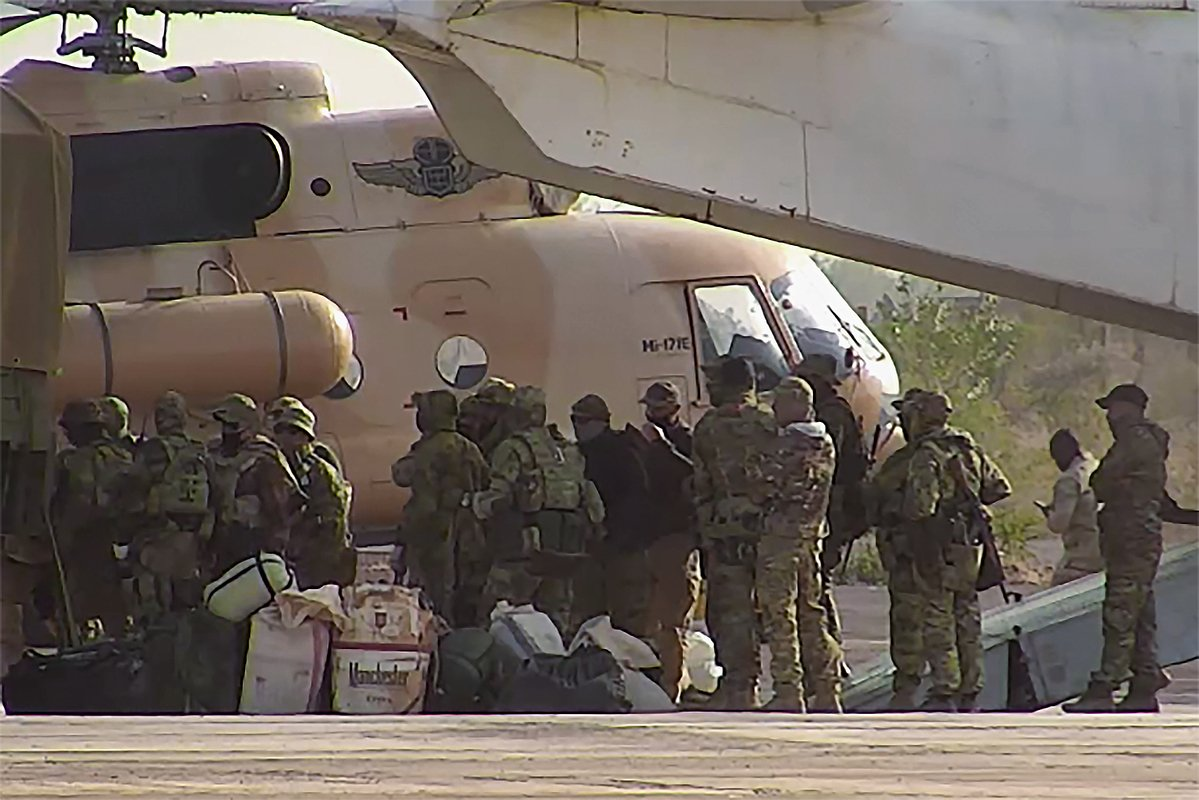
\includegraphics[width=0.75\textwidth]{img/pmc_africa_1.jpg}
    \caption{Предположительно сотрудники ЧВК «Вагнер» садятся в вертолет на севере Мали, фотография не датирована; Фото: French Army / AP}
\end{figure}

Также сообщалось, что за услугами «музыкантов» обращались различные политические силы в Ливии, Судане, Мозамбике, а также, возможно, власти Буркина-Фасо (хотя они это отрицают). По разным данным, в обмен структуры ЧВК «Вагнер», помимо финансового \ed{вознаграждения}{вознаграждение}{remuneration; compensation}, также получали доступ к добыче природных ресурсов в странах пребывания.

\begin{center}
    \Large

    Впрочем, министр иностранных дел России Сергей Лавров \ex{заверил}{reassured}, что никакой паники среди африканских коллег не заметил
\end{center}

Напротив, ряд африканских представителей связались с ним, чтобы выразить свою солидарность с российским руководством. По его словам, правительства Мали и ЦАР, помимо пригожинской ЧВК, поддерживают контакты с официальными властями, а несколько сотен военнослужащих, которые работают в ЦАР в качестве инструкторов, продолжат свою работу, несмотря на последние события.

При этом официальный представитель Министерства иностранных дел (МИД) России Мария Захарова уточнила, что решение о продолжении работы в Африке непосредственно специалистов ЧВК «Вагнер» будут принимать сами африканские страны. Также она подчеркнула необходимость отделять обычных бойцов от организаторов мятежа, призвав «смотреть не на trademark ``Вагнер'', не на термин, а на суть».

\begin{wrapfigure}{r}{0.5\textwidth}
    \begin{fancyquotes}
        Она заключается в том, что за последние годы люди это доказали, занимаясь на фронте, на передовой, обеспечением нашей безопасности (...) проявляли себя соответствующим образом в Сирии, в африканских государствах

        \begin{flushright}

            Мария Захарова\\

            пресс-секретарь МИД России
        \end{flushright}
    \end{fancyquotes}
\end{wrapfigure}
Однако непонятно, позволят ли бойцам оставаться в Африке под тем самым trademark «Вагнер». В своем обращении президент России Владимир Путин дал «музыкантам» выбор из трех вариантов: заключить контракт с Министерством обороны России или другим силовым органом, вернуться домой к родным или «уйти в Белоруссию».


\begin{center}
    \Large
    \ed{Затрагивают}{затрагивают}{affect} или нет эти слова и тех бойцов ЧВК «Вагнер», что находятся в Мали и ЦАР, непонятно
\end{center}


\begin{figure}[h]
    \centering
    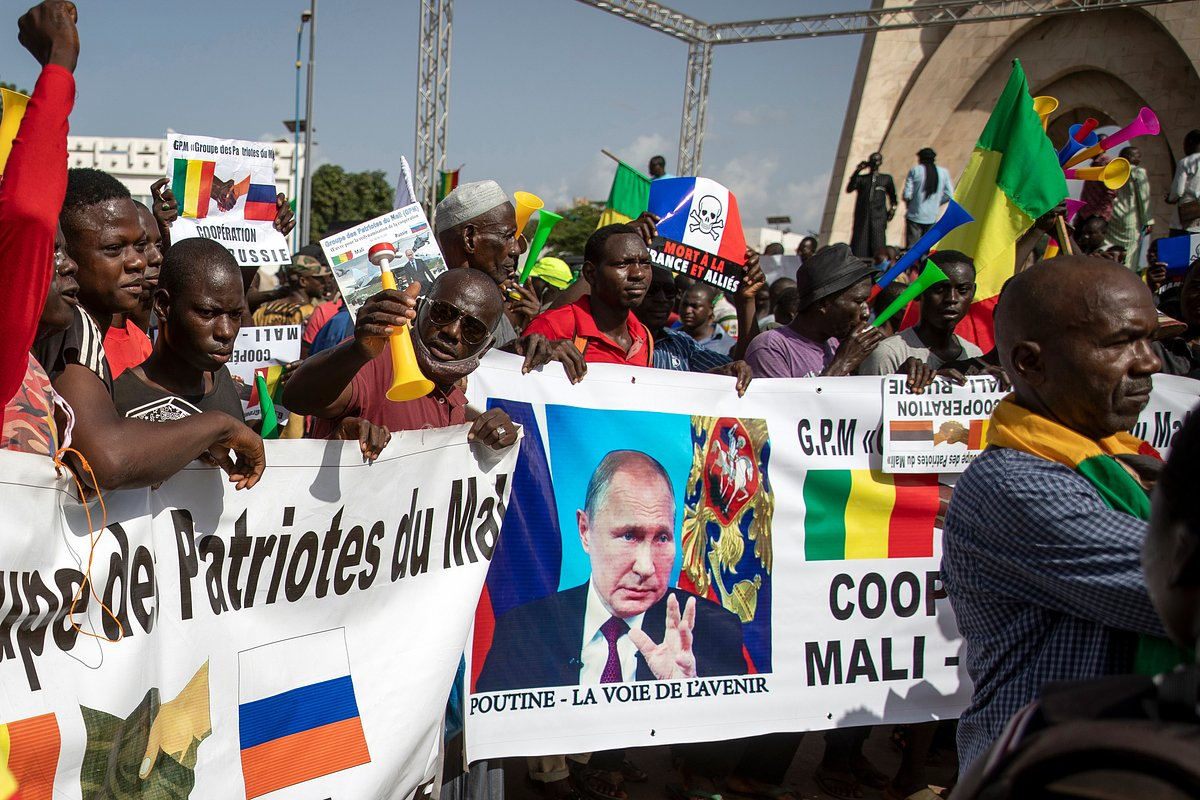
\includegraphics[width=0.75\textwidth]{img/pmc_africa_2.jpg}
    \caption{Жители Мали на демонстрации против Франции и в поддержку России по случаю 60-летия независимости страны, Бамако, 22 сентября 2020 года; Фото: AP }
\end{figure}

Более того, глава комитета Государственной Думы по обороне Андрей Картаполов заявил: отказавшиеся от подписания договоров формирования не будут получать «ни денег, ни финансовых, ни материальных ресурсов». Как отмечает The Financial Times, без материальной и логистической поддержки российских властей вагнеровцам будет крайне сложно продолжить работать в Африке.

\begin{center}
    {\Huge 86,3}\\
    {\huge млрд рублей}\\[1em]

    {\Large выплачено ЧВК «Вагнер» из госбюджета с мая 2022 года по май 2023 года }
\end{center}

«Лента.ру» направила запрос в пресс-службу Министерства обороны России с просьбой прояснить позицию ведомства по данному вопросу. На момент публикации материала ответа не поступило.

\begin{center}
    \Large Сам Евгений Пригожин не рассказывал, чем дальше будет заниматься его ЧВК «Вагнер» и сохранится ли ее африканское подразделение
\end{center}


\begin{figure}[h]
    \centering
    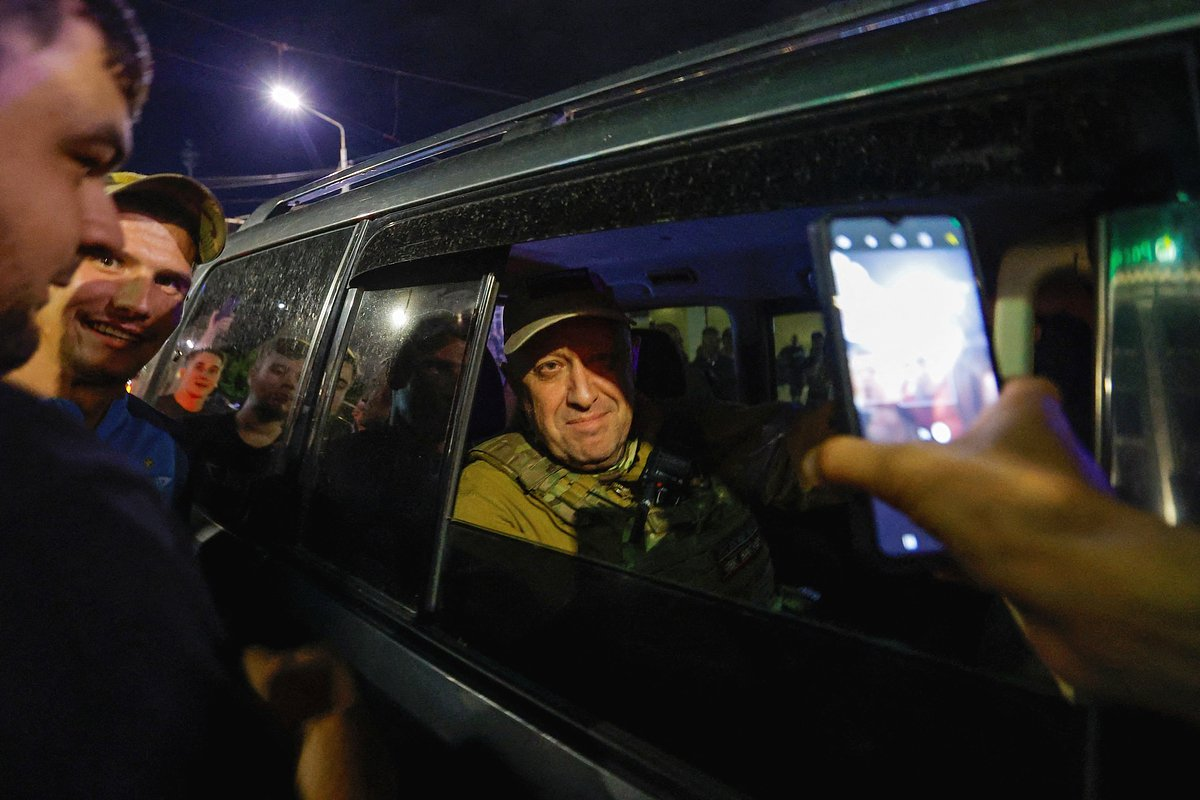
\includegraphics[width=0.75\textwidth]{img/pmc_africa_3.jpg}
    \caption{Евгений Пригожин покидает штаб Южного военного округа в Ростове-на-Дону, 24 июня 2023 года; Фото: Alexander Ermochenko / Reuters}
\end{figure}

Президент Белоруссии Александр Лукашенко, выступивший в качестве посредника между российскими властями и Евгением Пригожиным, заявил, что ушедшие в республику вагнеровцы могут быть привлечены к обучению местных подразделений.

Впрочем, пока дипломаты в ЦАР не заметили очевидных перемен в обстановке в стране после мятежа: представители ЧВК «Вагнер» были замечены в Банги и после событий 24 июня, сообщает The Financial Times. При этом местные власти уже выразили готовность принять от России любую военную помощь.

\begin{fancyquotes}
    Если Москва решит отозвать вагнеровцев и прислать вместо них «бетховенов» или «моцартов», мы будем не против

    \begin{flushright}
        Фидель Гуанджики\\
        советник президента ЦАР
    \end{flushright}
\end{fancyquotes}

The Financial Times отмечает, что речь может идти про другие российские ЧВК, \ex{предположительно}{presumably} связанные с «Газпромом».

Необходимо учитывать, что многие проекты ЧВК «Вагнер» в Африке были \ed{убыточными}{убыточный}{unprofitable} и \ed{дотационными}{дотационный}{subsidized}, то есть часть расходов на них прямо или \ex{к\'{о}свенно}{indirectly} компенсировалась из бюджета, отмечает директор Центра изучения Африки НИУ ВШЭ Андрей Маслов. По его словам, те проекты, где доходная база генерируется в самой Африке, могут претерпеть ребрендинг, тогда как дотационные проекты могут быть переданы под контроль Министерства обороны России и продолжить реализовываться в формате официальной поддержки по развитию местных вооруженных сил.

\begin{wrapfigure}{l}{0.5\textwidth}
    \begin{fancyquotes}
        Как показывает практика, такой формат более эффективен и несет в себе меньше рисков. Прямое сотрудничество имеет большие перспективы и более стабильно

        \begin{flushright}
            Андрей Маслов\\
            директор Центра изучения Африки НИУ ВШЭ
        \end{flushright}
    \end{fancyquotes}
\end{wrapfigure}
Африканист также призвал не \ex{переоценивать}{overestimate} роль ЧВК «Вагнер» --- и в архитектуре российско-африканских связей, и в архитектуре связей в области обороны и безопасности в регионе. Он напомнил, что Россия заключила официальные соглашения с десятками африканских государств, а в ЦАР по согласованию с ООН работают российские инструкторы от Министерства обороны России.

При этом масштаб деятельности ЧВК «Вагнер» в Африке сильно преувеличен как самой структурой и связанной с ней сеткой Telegram-каналов, так и западными чиновниками, которые запугивают африканцев и самих себя «ужасными русскими наемниками», полагает эксперт. Более того, ни Мали, ни ЦАР не входят в десятку ведущих африканских партнеров России по объемам торговли и инвестиций.

\begin{center}
    \Large
    Андрей Маслов предположил, что сотрудничество с Мали и ЦАР продолжится по линии Министерства обороны России — произойдет своего рода «национализация» программ содействия местным вооруженным силам
\end{center}

\begin{figure}[h]
    \centering
    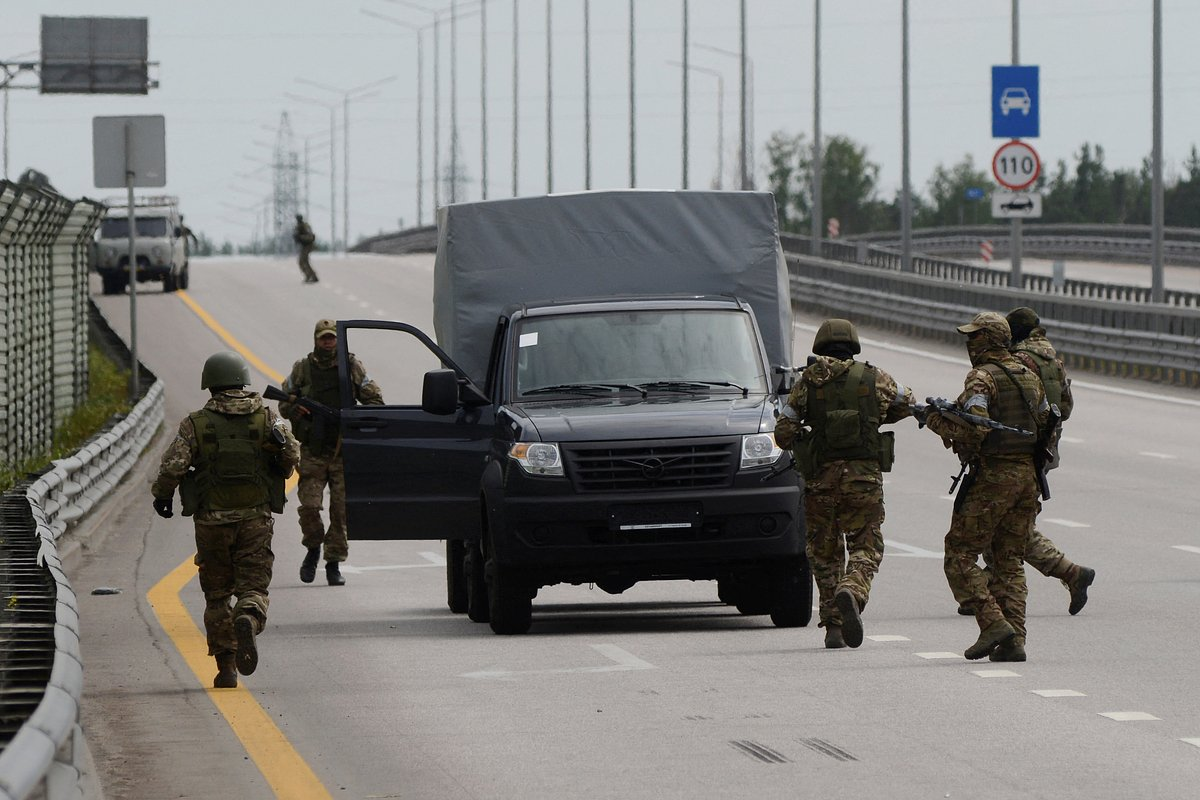
\includegraphics[width=0.75\textwidth]{img/pmc_africa_4.jpg}
    \caption{Бойцы ЧВК «Вагнер» обходят автомобиль на трассе М-4 недалеко от Воронежа, 24 июня 2023 года; Фото: Reuters}
\end{figure}

Что касается Мали, то Россия может быть заинтересована, например, в усилении роли Алжира в вопросах обеспечения безопасности в Сахаре, поскольку это североафриканское государство обладает значительным опытом в данной сфере и остается верным и крепким союзником России. Разумеется, сотрудничество с Алжиром никоим образом не должно идти в ущерб суверенитету Мали.

% -- <> -- 
\begin{fancyquotes}
    Поэтому российская сторона заинтересована в укреплении межгосударственных связей на региональном уровне и усилении африканского компонента в обеспечении безопасности. В долгосрочной перспективе это даст нам преимущества

    \begin{flushright}
        Андрей Маслов\\
        директор Центра изучения Африки НИУ ВШЭ
    \end{flushright}

\end{fancyquotes}

\textbf{Китайские стражи.} На африканском континенте, помимо ЧВК «Вагнер», работает множество частных военных компаний: американские CACI и Constellis, британские Aegis Defence Services и G4S, французская Secopex, немецкая Asgaard и многие другие.

\begin{center}
    \Large
    Специалисты затрудняются назвать даже примерное число иностранных наемников в Африке
\end{center}

Дело в том, что местные политические силы не любят афишировать свои связи с подобными структурами, а сами компании, как правило, заключают соглашения о неразглашении, запрещающие им делиться подробной информацией о характере их работы в африканских странах.

Впрочем, Андрей Маслов усомнился, что западные военные компании могут создать альтернативу ЧВК «Вагнер», поскольку изначально занимают другую нишу, работая с корпоративным сектором и занимаясь охраной объектов западных добывающих компаний. Африканские государства-заказчики же при выборе подрядчиков исходят из своих внешнеполитических приоритетов, а не из рыночных условий: что Мали, что ЦАР воспринимали ЧВК «Вагнер» как рекомендованную российским государством структуру.

\begin{fancyquotes}
    Какой частной она бы ни была, для Мали и ЦАР важно то, что она российская. Поэтому вряд ли произойдет вытеснение ЧВК «Вагнер» иностранными структурами на рыночных условиях


    \begin{flushright}
        Андрей Маслов\\
        директор Центра изучения Африки НИУ ВШЭ
    \end{flushright}

\end{fancyquotes}


\begin{figure}[h]
    \centering
    
\includegraphics[width=0.75\textwidth]{img/pmc_africa_5.jpg}
    \caption{Презентация технологии идентификации человека от государственного производителя оборудования для наблюдения Hikvision на выставке Security China 2018 в Пекине, Китай, 23 октября 2018 года; Фото: Ng Han Guan / AP}
\end{figure}

Особняком стоят частные охранные фирмы из Китая, начавшего масштабную экономическую экспансию на континент в рамках запущенной в 2013 году инициативы «Один пояс — один путь»: соответствующие соглашения подписаны с 52 из 54 африканских стран. К настоящему моменту в Африке работает около 10 тысяч китайских компаний и, по разным оценкам, от 1 до 2 миллионов китайских рабочих, задействованных в развитии инфраструктуры, строительстве жилья, промышленном производстве и добыче полезных ископаемых.

Однако обстановка с безопасностью в ряде африканских стран оставляет желать лучшего: на континенте орудуют многочисленные вооруженные группировки, для которых похищение иностранных рабочих — один из основных источников дохода. Рабочих из Китая считают лакомой добычей: китайские корпорации, как правило, не жалеют денег, чтобы вызволить своих сотрудников.

\begin{center}
    \Large
    Полагаться на местные органы безопасности не приходится, тем более с учетом довольно неспокойной внутриполитической обстановки в ряде стран Африки: китайские рабочие не раз оказывались буквально меж двух огней враждующих фракций
\end{center}

Все это подтолкнуло китайскую сторону к тому, чтобы самостоятельно заняться защитой своих граждан, благо есть кем: в Поднебесной зарегистрировано свыше пяти тысяч частных охранных компаний, в которых работает около четырех миллионов человек, преимущественно из числа бывших военных.

\begin{center}
    \Large
    Частные военные компании в Китае запрещены, а все охранные предприятия строго подконтрольны Министерству общественной безопасности КНР
\end{center}

За пределами Китая разрешено работать всего 20 компаниям, а в Африке работает по меньшей мере девять из них: Beijing DeWe Security Service, Hua Xin Zhong An Group, Shandong Huawei Security Group, China Security Technology Group, China Overseas Security Group, Frontier Services Group, China Overseas Security Service, VSS Security Group и Zhongjun Junhong Security Service.


\begin{figure}[h]
    \centering
    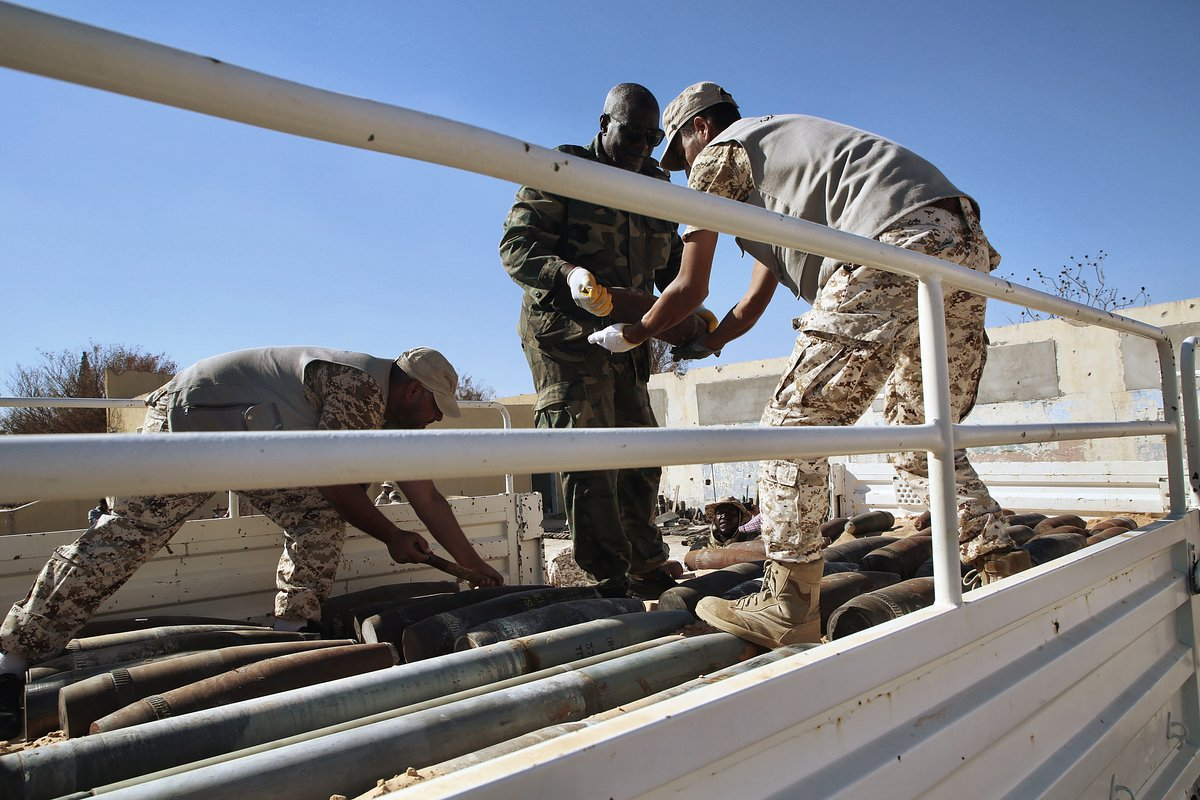
\includegraphics[width=0.75\textwidth]{img/pmc_africa_6.jpg}
    \caption{Ливийские ополченцы и специалсты из ЧВК «Вагнер» на погрузке боеприпасов, район Аль-Хира, в 75 километрах к югу от Триполи, Ливия, 22 июля 2020 года; Фото: Hazem Turkia / Anadolu Agency / Getty Images}
\end{figure}

По официальным данным, за границей работают всего 3200 сотрудников китайских частных охранных фирм, но исследователи полагают, что цифры сильно занижены: в одной лишь Кении защитой строительства железной дороги Момбаса — Найроби — Найваша занималось 2000 сотрудников DeWe.

Василий Кашин, директор Центра комплексных европейских и международных исследований НИУ ВШЭ и специалист по китайскому военно-промышленному комплексу, отмечает, что подавляющему большинству подобных фирм запрещено пользоваться оружием. Исключение составляют сотрудники Overseas Security Guardians и Hua Xin Zhong An Group, которые обеспечивают вооруженный конвой для китайских судов, следующих в африканских водах.

В остальных случаях сотрудники подобных фирм организуют охрану китайских предприятий с помощью нелетальных вооружений, решают технические задачи и выстраивают партнерство с местными охранными структурами. «А задачи, требующие использования оружия, они решают как раз за счет найма местных партнеров», — рассказал Василий Кашин в беседе с «Лентой.ру».

Например, в июле 2016 года DeWe прибегла к найму местных вооруженных сотрудников, чтобы эвакуировать свыше 300 китайских нефтяников из южно-суданской столицы Джубы, в которой разгорелось вооруженное противостояние между правительственными и оппозиционными силами.

Таким образом, китайские охранные предприятия значительно отличаются от структур ЧВК «Вагнер» — и по своему устройству, и по своим задачам, а потому вряд ли станут альтернативой российской компании в случае ее ухода с континента, считает специалист.

\begin{fancyquotes}
    Китайцам страшно помыслить о том, чтобы разрешить своему охранному бизнесу заниматься тем же, чем занимался «Вагнер»

    \begin{flushright}
        Василий Кашин\\
        директор Центра комплексных европейских и международных исследований НИУ ВШЭ
    \end{flushright}
\end{fancyquotes}

\textbf{Новые башибузуки.} Еще один игрок на африканском континенте, который может воспользоваться уходом вагнеровцев, — турецкая частная военная компания Sadat International Defense Consultancy, основанная в 2012 году. На официальном сайте утверждается, что SADAT — это «первая и единственная частная ЧВК в Турции, которая на международном уровне предоставляет услуги консалтинга, военной подготовки и логистики в секторе международной обороны и внутренней безопасности».

\begin{center}
    \Large
    Одним из главных преимуществ турецкой ЧВК SADAT считается наличие «готовых военно-воздушных сил», вооруженных беспилотниками Bayraktar, зарекомендовавшими себя в конфликтах на Украине, в Нагорном Карабахе и Ливии
\end{center}

\begin{figure}[h]
    \centering
    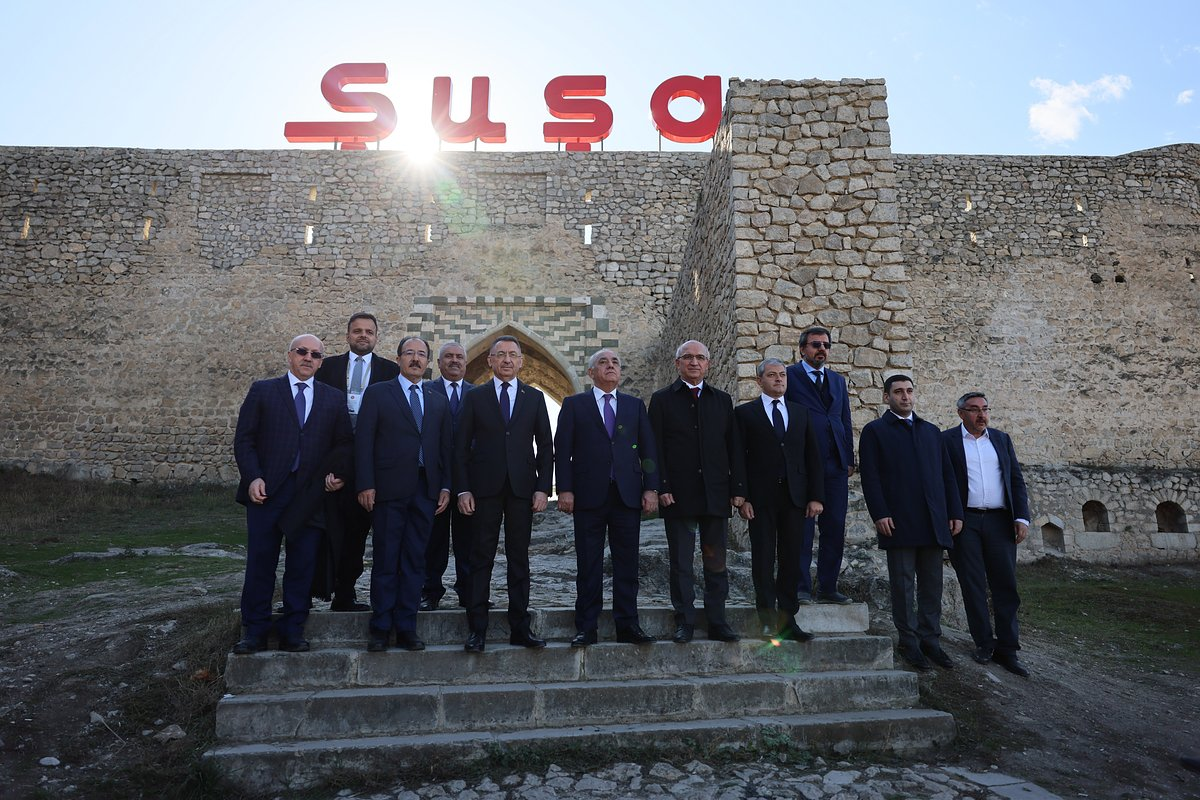
\includegraphics[width=0.75\textwidth]{img/pmc_africa_7.jpg}
    \caption{Вице-президент Турции Фуат Октай и премьер-министр Азербайджана Али Асадов посещают город Шуша в Нагорном Карабахе, Азербайджан, 5 ноября 2022 года; Фото: Berke Bayur / Anadolu Agency / Getty Images}
\end{figure}


Ряд наблюдателей считает SADAT личной армией президента Турции Реджепа Тайипа Эрдогана. Во время попытки госпереворота в июле 2016 года бойцы SADAT участвовали в подавлении протестов и, вероятно, даже стреляли по гражданским, рассказывает старший научный сотрудник American Enterprise Institute Майкл Рубин. С 2016 по 2022 год основатель SADAT Аднан Танрыверди также занимал пост главного военного советника турецкого лидера. При этом сам Реджеп Эрдоган опровергает всякие обвинения в покровительстве ЧВК.

По различным данным, SADAT работает в Сомали и Катаре, сотрудничала с палестинским движением ХАМАС и обучала ливийских повстанцев и сирийских боевиков, выступавших против правительства Башара Асада, в том числе якобы завербованных на Кавказе бойцов «Исламского государства» и «Джебхат ан-Нусры» (террористическая группировка, запрещенная в России).

ЧВК, вероятно, также была активно задействована и в конфликте в Нагорном Карабахе осенью 2020 года. По сведениям газеты «Коммерсант», SADAT занималась вербовкой и подготовкой сирийских боевиков на подконтрольных Турции территориях на севере и северо-западе Сирии, после чего обученных наемников — около 1,3 тысячи бойцов — перебросили в зону конфликта на чартерах, зафрахтованных все той же SADAT.

Кроме того, осенью 2022 года сообщалось о планах ЧВК направить своих наемников в Кашмир, являющийся предметом территориального спора между Индией и Пакистаном.

\begin{center}
    \Large
    В самом SADAT настаивают, что не участвуют в конфликтах в качестве наемников, а оказывают исключительно консультационные и образовательные услуги
\end{center}


\begin{figure}[h]
    \centering
    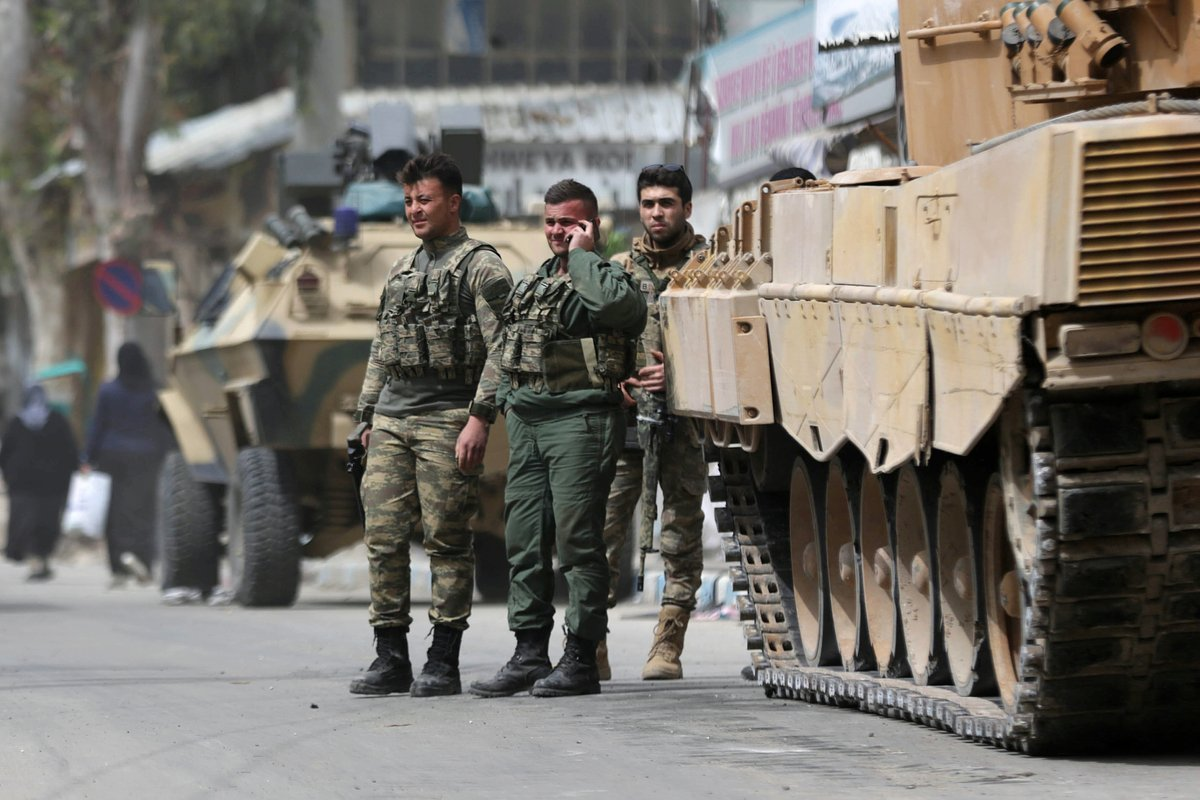
\includegraphics[width=0.75\textwidth]{img/pmc_africa_8.jpg}
    \caption{Турецкие солдаты в центре Африна, Сирия, 24 марта 2018 года; Фото: Khalil Ashawi / Reuters}
\end{figure}

Как и многие другие страны, в последние годы Турция активно развивает официальные связи с Африкой: страна значительно расширила свою сеть посольств на континенте, а ее президент посетил больше африканских государств, чем кто-либо из неафриканских лидеров.

Особое внимание уделяется наращиванию военно-технического сотрудничества с Африкой: лишь за 2021 год поставки турецкого военного оборудования на континент выросли в пять раз, правда, занимают пока меньше одного процента от рынка. Впрочем, этот показатель, вероятнее всего, продолжит расти — не в последнюю очередь благодаря растущей популярности турецких дронов Bayraktar.

Помимо Ливии, турецкие военные присутствуют в Сомали, где обучают местных солдат и офицеров военному ремеслу, причем на турецком языке, а сомалийские новобранцы даже приносят присягу сразу на двух языках. Кроме того, турецкие военнослужащие задействованы в миротворческих миссиях ООН в Демократической Республике Конго, Мали, Сомали, Судане, Южном Судане и ЦАР.

Впрочем, основатель SADAT Аднан Танрыверди еще в 2019 году призвал к переменам: по его словам, Турции необходимо создать полноценный аналог американской Blackwater, бойцы которой отправятся выполнять военные задачи в Африку, тогда как официальные вооруженные силы сосредоточатся на обороне собственной страны.

\begin{fancyquotes}
    Турция имеет глубоко укоренившиеся военные традиции. ЧВК могут оказывать услуги дружественным странам, нанимая отставных и недавно демобилизованных солдат. А затем их можно будет использовать как инструмент внешней политики

    \begin{flushright}
        Аднан Танриверди\\
        основатель SADAT
    \end{flushright}
\end{fancyquotes}

Впрочем, чтобы отказаться от услуг россиян в пользу турков, африканские государства, где сейчас работает ЧВК «Вагнер», должны будут сначала изменить свой политический курс, отмечает Андрей Маслов.

\begin{fancyquotes}
    Но пока предпосылок к тому, чтобы ЦАР или Мали поменяли свой внешнеполитический вектор, мы не видим

    \begin{flushright}
        Андрей Маслов\\
        директор Центра изучения Африки НИУ ВШЭ
    \end{flushright}
\end{fancyquotes}

Сам основатель SADAT Аднан Танрыверди другим важным условием считает разработку турецкими властями законодательства, которое бы устанавливало контроль государства над будущими военными компаниями. Мятеж Евгения Пригожина, вероятно, может ускорить этот процесс. Впрочем, все те же события 24 июня могут заставить Реджепа Эрдогана, наоборот, более настороженно отнестись к легализации и расширению сферы деятельности ЧВК — тем более что в 2016 году он уже пережил одну попытку госпереворота.

Китайские и турецкие ЧВК вряд ли сумеют составить достойную альтернативу ЧВК «Вагнер» в обозримом будущем: и в силу их текущей структуры и сфер деятельности, и в силу того, что сами Китай с Турцией, по всей видимости, не особо к этому стремятся. Западные ЧВК тоже не смогут претендовать на нишу вагнеровцев — их клиенты в основной своей массе крайне негативно относятся к перспективе сотрудничества с «неоколониальными силами» и изначально обратились к россиянам именно из этих соображений.

\begin{center}
    \Large
    Наконец, не похоже на то, что Россия сама готова отказаться от целого измерения сотрудничества со странами континента
\end{center}

Вероятно, российские власти выработают какое-то решение, которое позволит специалистам ЧВК «Вагнер» и дальше оказывать свои услуги в странах Африки в обмен на определенные гарантии лояльности. А уж под каким брендом — особой роли не играет: в африканских странах дали четко понять, что будут рады любым российским «музыкантам» — хоть «бетховенам», хоть «моцартам».

\newpage
\section{Караганов призвал Кремль нанести ядерный удар по Польше}

\textit{Спецкор «Медузы» Андрей Перцев объясняет, почему эти угрозы на самом деле опаснее, чем оголтелые посты Дмитрия Медведева}

\textit{Источник: \url{https://meduza.io}}
% https://meduza.io/feature/2023/06/15/politolog-sergey-karaganov-prizval-kreml-nanesti-yadernyy-udar-po-polshe

\textit{Журнал «Профиль» опубликовал — а издание «Россия в глобальной политике» перепечатало — статью политолога Сергея Караганова, суть которой сводится к тому, что Россия «должна нанести превентивный ядерный удар по Европе», чтобы «сломить волю Запада» и \explain{добиться победы}{achieve victory; добиться + чего} в войне с Украиной. Угрозы применения ядерного оружия со стороны Москвы звучат буквально с первых недель полномасштабной агрессии (этим занимается и сам Путин). Тем не менее статья Караганова, к сожалению, выглядит не просто очередным сотрясанием воздуха. \ed{Спецкор}{спецкор}{специальный корреспондент} «Медузы» Андрей Перцев объясняет почему.
}

\textbf{Кто такой Сергей Караганов? И почему его статья вообще \explain{заслуживает внимания}{deserved attention}?}

Доктора исторических наук и политолога Сергея Караганова вы, возможно, помните по проекту «\ed{Намедни}{нам\'{е}дни}{на днях; недавно}. Наша эра» журналиста Леонида Парфенова. Он комментировал советскую политическую историю — и делал это во вполне либеральном ключе. Еще в 2011 году Караганов, например, проповедовал «декоммунизацию» и «десталинизацию».

С тех пор многое поменялось. Сейчас Сергей Караганов --- один из основателей российского Совета по внешней и оборонной политике (СВОП). Это экспертный центр, с которым сотрудничают бывшие военные, дипломаты, действующие политики, исследователи и журналисты. В 2004 году СВОП стал одним из учредителей клуба «Валдай», в заседаниях которого регулярно участвует Путин. Сам Караганов, разумеется, тоже посещает эти встречи. Заседания клуба модерирует его соратник по СВОП, журналист-международник и политолог Федор Лукьянов. Он же возглавляет журнал «Россия в глобальной политике», а Караганов руководит редакционным советом издания.

\begin{wrapfigure}{l}{0.45\textwidth}
    \centering
    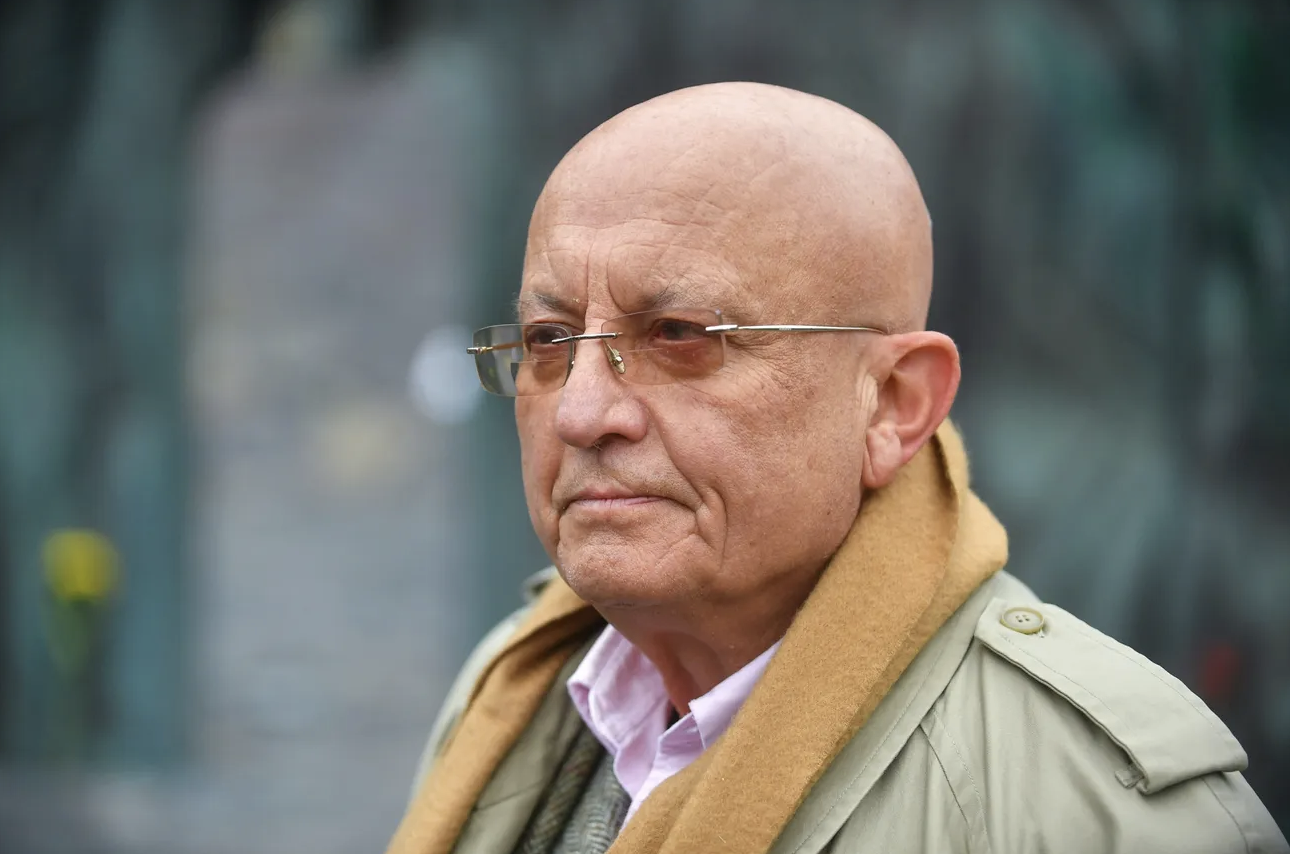
\includegraphics[width=0.43\textwidth]{img/karaganov.png}
    \caption{Сергей Киселев / Агентство «Москва»}
\end{wrapfigure}
У Караганова есть еще одна высокая регалия --- научный руководитель факультета мировой экономики и мировой политики Высшей школы экономики. Но самое главное, что он входит в состав научного совета при Совете безопасности РФ, который на фоне вторжения стал, по всей видимости, ключевым органом власти в России. Два источника «Медузы», близких к администрации президента (АП), называют Караганова человеком, который «может влиять на мнение секретаря Совбеза Николая Патрушева». А тот, в свою очередь, как считается, входит в близкий круг Путина.

Впрочем, третий собеседник «Медузы», близкий к Кремлю, призывает «не преувеличивать влияние Караганова». Тем не менее политолог реально участвует в деятельности Совета безопасности РФ и регулярно бывает на мероприятиях с участием Путина.

По косвенным признакам можно предположить, что руководители силового блока как минимум знакомы с идеями Караганова, а может быть, даже \explain{вдохновляются}{are inspired} ими. Вы наверняка слышали эксцентричные высказывания Николая Патрушева и главы Службы внешней разведки Сергея Нарышкина о том, что Польша «готовится захватить украинские земли» (подробнее об этом читайте, например, \href{https://carnegieendowment.org/politika/88530}{тут}). Так вот: Караганов \href{https://globalaffairs.ru/articles/rakety-v-evrope-vospominaniya-o-budushhem/}{рассуждал} об этом еще в 2016 году:

\begin{fancyquotes}
    Она (Украина) вряд ли может состояться как государство в долгосрочной перспективе. Скорее всего, страна будет медленно распадаться. Ну а там история покажет. Не исключено, что что-то может отойти к России, что-то — к Венгрии, что-то — к Польше, а что-то может остаться формально независимым Украинским государством.
\end{fancyquotes}

\textbf{Дмитрий Киселев в прямом эфире грозил превратить США в «радиоактивный пепел» еще до аннексии Крыма. А недавно ядерным ударом пугал Запад Дмитрий Медведев. Неужели слова политолога Караганова значат больше?}

В каком-то смысле да. Дмитрий Киселев в середине 2010-х был главным пропагандистом российской власти. В этом качестве он театрально и, \explain{по всей видимости}{apparently}, совершенно \explain{осознанно}{consciously} \explain{эпатировал}{shocked, scandalised} либерально настроенных \ed{сограждан}{согражданин}{fellow citizen} --- выступая с речами, вызывающими ужас и стыд, но не имеющими никаких последствий. Примерно тем же (несмотря на свой прежний и нынешний\footnote{Формально бывший президент и бывший премьер Медведев остается заместителем Путина в Совбезе РФ. Эту должность придумали специально для него, чем он там занимается, неизвестно.} высокий статус) занимается и Медведев, который в своем телеграм-канале оскорбляет западных политиков и жителей других стран.

В случае Киселева и Медведева угрозы ядерным оружием воспринимаются в ряду других не менее жестких заявлений. В отличие от Киселева и Медведева, Караганов всегда вел себя сдержанно. При этом его статья перепечатана в журнале «Россия в глобальной политике»: это медиа когда-то было запущено по модели западного аналитического издания при участии американского журнала Foreign Affairs — и до последнего времени считалось серьезным и уважаемым. Даже после 24 февраля журнал не исключили из международных баз данных научных публикаций (например, Scopus), то есть публиковаться там, в том числе зарубежным ученым, по-прежнему допустимо и даже — теоретически — престижно.

Статью Караганова, вероятно, можно воспринять как личную инициативу, попытку послать сигнал высшему руководству страны — и предложить свой радикальный вариант выхода из кризиса, в котором Россия оказалась из-за военной агрессии против Украины. С другой стороны, учитывая близость Караганова к Совбезу РФ и его личное участие в организации «Валдая», этот текст вполне может транслировать мнение, распространенное в силовом — самом влиятельном — блоке российской власти.

\textbf{То есть это статья написана лично для Путина?}

Возможно. \ed{В пользу}{в пользу}{in favour} этой версии говорит риторика, которую использует Сергей Караганов. Она очень близка российскому президенту: политолог явно пытается соответствовать путинскому языку. Например, в тексте встречается «пацанская аргументация», характерная для президента РФ: в частности, когда Караганов объясняет, что превентивный ядерный удар по Европе нужен, «чтобы Запад просто ``отвалил'' и не мешал\footnote{мешать + кому} России и миру идти вперед». Не забыл Караганов упомянуть и «неоколониализм», который в последние полтора года \explain{к месту}{in place} и не к месту вспоминает Путин.

Или вот еще одно, по сути, повторение излюбленных путинских клише:

\begin{fancyquotes}
    Запад теряет имевшуюся у него на протяжении пяти веков возможность \ex{высасывать}{suck} богатство из всего мира, \ed{навязывая}{навязывать}{to impose}, в первую очередь грубой силой, политические, экономические порядки и устанавливая свое культурное доминирование. Так что быстрого окончания развертываемой Западом оборонительной, но агрессивной конфронтации ожидать не приходится.
\end{fancyquotes}

Караганов вспоминает также «отрицание семьи, родины, истории, любви между мужчиной и женщиной, веры, служения высшим идеалам, всего того, что составляет сущность человека» --- все это, разумеется, на Западе. Узнаете? Да, Путин тоже об этом много и часто говорит.

При этом автор успокаивает своего потенциального высокопоставленного читателя --- того самого, который гипотетически может принять решение о применении ядерного оружия: США якобы не \ed{вст\'{у}пятся за}{вступ\'{и}ться за кого-либо}{to stand up for} Европу, никто не будет жертвовать «условным Бостоном ради условной Познани». Караганов \ex{подкрепляет}{reinforces} эту мысль еще одним опасным тезисом: «Победителей не судят, а спасителей благодарят». А что победа в итоге окажется за Россией, как бы само собой разумеется.

Насколько лет назад Караганов доказывал, что ядерное оружие, которым располагает Россия, было залогом отказа Запада от поставок оружия Украине во время войны в Донбассе 2014–2015 годов:

\begin{fancyquotes}
    Когда горячие головы в Вашингтоне требовали поставки Киеву «летальных вооружений», европейцы, да и руководство США категорически это \ex{отвергли}{rejected}, поскольку понимали, что Россия, прикрытая ядерным оружием и обретшая волю к борьбе, ответит крайне жестко.
\end{fancyquotes}

Но теперь, когда США и страны Евросоюза такое вооружение поставляют, получается, что Россия просто «обязана» сделать следующий опаснейший шаг.

Если Караганов (один или вместе с влиятельными единомышленниками) действительно хочет убедить президента РФ в необходимости нанести ядерный удар, вполне логично, что он доносит эту мысль в приятной и знакомой Путину обертке.

\textbf{Довольно пугающая версия. А другие есть?}

Да. Возможно, Караганов пытается не убедить Путина ударить по Европе, а напугать влиятельных и высокопоставленных людей на Западе самой этой возможностью --- и склонить их к изменению позиции по Украине.

Здесь нужно еще раз вспомнить об эволюции взглядов политолога. Даже после аннексии Крыма их еще можно было назвать относительно миролюбивыми. В 2016 году Караганов предлагал российским властям такую программу:

\begin{fancyquotes}
    Лучше бороться за мир, \ex{выступать поставщиком безопасности}{act as a security provider}, в том числе предотвращая дальнейшую экспансию западных союзов, что мы, хотя и \ex{с запозданием}{belatedly}, сделали в 2014 г. [аннексировав Крым], срывать планы тех, кто хочет вернуть гонку вооружений и системный военно-политический конфликт, восстановить лидерство в борьбе за верховенство международного права, за стратегическую стабильность.
\end{fancyquotes}

Тогда политолог был уверен, что «планов по завоеванию Украины у нас точно нет». Однако уже в 2017 году Караганов начал фокусировать внимание на том, что «одной из основ формирования нового миропорядка» может стать диалог США, России и Китая по вопросу о ядерном сдерживании. Иными словами, он стремительно разуверился в идее борьбы за мир и «верховенстве международного права» и пришел к выводу, что ядерное оружие — более надежный гарант мира на планете, чем договоренности и принципы:

\begin{fancyquotes}
    «Большая тройка» будет закладывать основы для менее хаотичной и более безопасной мировой системы будущего. Этот новый «концерт наций», если и когда у лидеров трех стран хватит чувства ответственности создать его, может оказаться более устойчивым, чем предыдущий из XIX века, если он по согласию будет базироваться на взаимном ядерном сдерживании, а не только на моральных принципах или балансе сил.
\end{fancyquotes}

То есть уже как минимум шесть лет Караганов уверен, что только страх перед использованием ядерного оружия может удержать человечество от кровопролитной глобальной войны, — и пытается убедить в этом своих читателей.

Нынешняя статья продолжает эволюцию взглядов политолога. Если в 2017 году Караганов еще предлагал сторонам спокойно подумать о переговорах, то теперь он пытается посеять у читателей на Западе страх и заставить их согласиться на уступки.

Караганов, очевидно, надеется, что в западных странах заметят: теперь им угрожает не потерявший влияние бывший президент (выбравший в качестве публичной стратегии оскорбления в адрес всего, чем раньше сам восхищался) и не штатный пропагандист в популярном вечернем шоу (которому полагается выступать с самыми радикальными идеями). К ним со страниц авторитетного — как, очевидно, полагают в редакции — журнала обращается серьезный эксперт, который не так уж давно считал ядерный конфликт маловероятным.

Вероятно, с точки зрения Караганова, это должно послужить лишним аргументом, чтобы Запад наконец отказался от поддержки Украины. В статье такой вариант прямо проговаривается: «Все-таки велика вероятность, что удастся победить, образумить противника без крайних мер, заставить его отступить».

Иными словами, сам Караганов может считать свой текст дополнительным элементом «ядерного сдерживания».

\textbf{Но если статья Караганова — не более чем его личное послание (хоть Путину, хоть Западу), то бояться все равно нечего?}

К сожалению, даже в этом случае появление такой статьи — плохая новость. Во-первых, не будем забывать, что у автора могут быть влиятельные единомышленники. Во-вторых, слишком логичными и убедительными могут казаться Путину и его окружению рассуждения Караганова о ходе исторического процесса: Запад «умирает и теряет влияние»; его нужно огорошить мощным ударом; история будет «на нашей стороне».

Даже если цель Караганова только в том, чтобы напугать Запад, его статья вполне способна повлиять на решения руководства России. Из-за стремления звучать в унисон с Путиным текст может оказаться не элементом ядерного сдерживания, как, возможно, надеялся сам автор, а ступенькой вверх по лестнице ядерной эскалации.

Правда, аналитик британского исследовательского центра Chatham Housе Кеир Джайлс предлагает относиться к ядерным угрозам, звучащим из России, исключительно как к методу психологической войны. Как отмечает Джайлс, Кремль прибегает к этому методу всякий раз, когда у российской армии возникают реальные проблемы на фронте (а статья Караганова появилась вскоре после начала украинского контрнаступления). Но и Джайлс признает: Путин действительно ориентируется на пропагандистские СМИ и лояльных экспертов, и это может роковым образом влиять на решения президента РФ.

Вот понятный пример. Перед полномасштабным вторжением в Украину верхушка ФСБ убеждала Путина, что украинцы с цветами встретят российских солдат. Причем не факт, что все «ястребы» сами хотели большой войны — скорее, стремились угодить главе государства. Но в итоге, оперевшись на эти высказывания и оценки, Путин начал реальную агрессию.

Теперь игра, затеянная Карагановым с не самыми ясными намерениями, вполне может показаться руководству России планом легкой победы.